\documentclass{article}
\usepackage{graphicx}
\usepackage[utf8]{inputenc}
\usepackage{url}
\usepackage{natbib}
\bibliographystyle{agsm}

\graphicspath{ {./images/} }

\title{Dissertation}
\author{Quentin Sonnefraud}
\date{July 2020}

\begin{document}

\maketitle

\tableofcontents

\section{Setup Of Rebench Data}

\#\#\# Part to modify and develop

First thing I did was take the data collected  which is produced by rebench \cite{ReBench:2018}

It's a bit complicated to manipulate the data from the rebenchdb project so I took two days to do crud and a mapping rest of the database I deployed the HTTP server on https://api.rebench.vatoth.dev/ which allows me to manage the data more efficiently.

To deploy the application, I use Docker; this is an open-source software platform to create, deploy and manage containers a container image is. It is a set of light and independent software processes, gathering all the files necessary for the execution of the processes: code, runtime, system tools, library and parameters. They can be used to run Linux or Windows applications. So I dockerised the app to make it easier to deploy in the future. I also use docker-compose, it's a tool that allows to describe (in a YAML file) and manage (in the command line) several containers as a set of inter-connected services. In this application, I describe a set composed of 3 containers: Postgresql, the server node.js for the REST API and a python notebook to present the data. In the beginning, Docker was only used to manage the local working environment, for example, dependencies like PostgreSQL, which allowed me to separate the data from other databases on my computer.

The stack of the project in production is launched like this in production; it builds and launches Docker and does the network mapping between them.

docker-composes -f docker-composes.yml -f docker-composes.production.yml up --build -d

You can see the docker-compose-.yml file in the Github repository \url{https://github.com/Vatoth/master-thesis}. 



\section{Introduction}


\section{Warmup analysis}

\subsection{JIT}


So my understanding of Just in time compilation is that dynamically adapts to the current software workload, compiling "hot" code, i.e. the most used code at a given time (which may represent the entire program, but often only certain parts of the program are processed by Just in time compilation). Obtaining optimised machine code is much faster (normally from bytecode than from source code. Since the deployed bytecode is portable, Just in time compilation is possible for any architecture, provided that a JIT compiler is available for that architecture, which is facilitated by the fact that bytecode to machine code compilers is more comfortable to write than source code to native code compilers.

\subsection{\cite{barrett2017virtual}}

The idea behind this is to add a feature to automatically detect multiple states of the benchmark if it has warmup, flat, slow down or no steady-state \cite{barrett2017virtual}. 

So I used the experience done in this paper to get this feature.

\subsection{Clean outliers}

I applied python rolling windows to remove the tools in the benchmarks like the garbage collection.

\#\#\# Include plot and comment about outliers cleaning, find smarter ways than rolling windows

Anomaly detection consists in highlighting data with a different behavior from the majority of the data. In general, these
particular data are in the minority and their detection can be done according to all three known paradigms in machine learning. Indeed, the detection can be performed in supervised mode in case information on the normality of the data is available. In other words, any data in the learning base can be labeled as normal or abnormal. In semi-supervised mode, the training database is assumed to contain only normal data. 
As for the detection in unsupervised mode, no information on the normality of the data is available. 

\subsubsection{Unsupervised techniques}
The unsupervised approach is the most suitable for anomaly detection problems and benchmarks data. In this approach, the different algorithms try to distinguish aberrant observations by learning about the data set, without having the labels of the observations: there is no set of observations identified a priori as anomalies. It is therefore not necessary to have labelled data and this simplifies the problem of preparing the data before learning and all the difficulty in constructing labels. In this section, I will briefly present some unsupervised techniques and their application with Rebench Data.




\subsection{Classification}

There was some problem with the classification I adapted the algorithm which works now depending on the size of the benchmarks


\#\#\# Explain what i Did for get it working for rebench data maybe some pseudo code ????

\section{Overview of some changepoint detection algorithm and application of classifcation of warmup analysis}


So first I used a package which allows me to do changepoint analysis which is called ruptures \cite{truong2020selective}, it works well, but after reading the warmup paper I prefer to use the algorithm from R "changepoint" \cite{killick2014changepoint} in order to reproduce the experiment.

\subsection{Changepoint Detection}
In statistical analysis, the break detection problem is a regression problem to estimate the times at which a signal exhibits changes in the distribution. . Classically, changepoint detection is performed for a signal with changes in the mean. More generally, changepoint detection is performed for a signal with changes in the distribution (for example, in the mean and variance). \\

Changepoint  detection can be applied to a sound signal of a program for which we wish to estimate the moments when situations change, to the detection of computer attacks  , or to quality control, here for the rebench Data it help to classify behaviour in warmup analysis. \\

This next will deals with the problem of detecting breaks retrospectively (known as offline) when all the signal data are available. This context is different from a real time detection (online) where the signal data arrive on the fly it could be interessting to classify on the fly after reaching  and classifying a stabilisation of a benchmark and stoping recording the benchmark data in order to save time , but online detection is less able to detect precisely the moment of rupture.

\subsection{Offline detection Parametric and Non Parametric}
 
 
Theire two big families of offline detection algorithm

\subsubsection{Parametric}

Advantages: speed of calculation, ease of interpretation and prediction,
good speed of convergence, possibility of validation;
Disadvantages: a priori choice of known functions (example: degree of polynomial), adapted to a limited class of tendencies.

\subsubsection{Non-parametric:}


I Advantages: adaptability, not a priori on the type of trend;
I Disadvantages: limits in interpretation, validation and prediction,
choice of window / smoothing parameters.

\subsection{Package changepoint}

\#\#\# Include benchmarks

Of course, there are very different ways of proceeding to analyze this type of signal. One of the most "intuitive" is to cut the series into "homogeneous" segments. This notion of homogeneity can cover, for example, homogeneity in mean, or homogeneity in variance (or homogeneity in mean-variance!).

There is 3 type of detection of Changepoint
Changepoint in mean, Changepoint in variance, and Changepoint mean or variance

\#\#\# Include bencmarks with noise and changement in mean and variance


For example, for the three benchmarks above, it looks like:

the x1 series is affected by changes in the average,
the x2 series is affected by changes in variance, and
the x3 series by changes in mean and variance.

Based on these models, here is the kind of segmentation that could be proposed:

The above results are actually obtained using the changepoint package from Killick and Eckley (2011).

I used 3 different functions:

cpt.mean which is used to detect breaks in the mean (assuming that the variance is constant)
cpt.var which is used to detect breaks in the variance (assuming that the mean is constant)
cpt.meanvar which is used to detect breaks in both the mean and the variance
These three functions are largely configurable. One can thus vary (among others)

The nature of the algorithm used to detect "optimal" breakpoints...
the type of test used to locate the breaks (one can either assume that the residual distribution of the variables is Gaussian, or one can not make an assumption of distribution and use a non-parametric test)
the type and extent of the penalty applied in order to limit over-segmentation.

These aspects are discussed in Killick and Eckley (2014).

Effect of parameterization

Unsurprisingly, the above functions give very different results depending on how you set them up .

For example here, I can vary the type of algorithm:

\#\#\# Include bencmarks with noise and changement in mean and variance change algorithm

Here I vary the cost function fixed mannualy:

\#\#\# Include bencmarks with noise and changement in mean and variance change cost function

How do I choose a method?
To choose the segmentation algorithm and other associated parameters, we will rely on 3 criteria:

theoretical criteria (which model is best suited to your data? one with constant variance, one where the residuals are Gaussian, one that would account for segments of highly variable lengths, etc.).

Empirical criteria (we choose the method that gives the most "usable" results on real data, and the most correct results on simulated data). This is what i used because i assume that the data from \cite{barrett2017virtual} was verrified and are correct.

Calculation criteria (the method must be computationally applicable for data of a certain size).

Obviously, determining which method is best using multiple criteria of these three types is difficult (if not impossible). Nevertheless, it is possible to discuss it by carrying out (perhaps, all the same, less ambitious!!) the same type of study as \cite{leviandier2012comparison}.


\subsection{Exact segmentation: dynamic programming}



\section{ How to detect the change between benchmarks ? Overwiew of method to quantify difference between curve}

DUring this project I have review and try some techniques to quantify the difference between benchmarks and report if changement of behavior as occure

\subsection{Area method}

First i have used area method to quantify the difference between curve, this an algorithm for calculating the Area between two curves in 2D space
Strictly speaking, the expression area under the curve refers to the area A of the domain delimited by a curve (represented in an x-y diagram) and three straight lines (the x-axis and two vertical lines with abscissa a and b). If the curve has the equation $y=f(x) y=f(x)$, the area is $A=\int _{a}^{b}f(x)\, {d} x$. This area is a true area (e.g. milliseconds for benchmarks) only if the function f has only positive (or zero) values over the interval [a,b] and if both the abscissa and the ordinate are lengths (with the same choice of unit, e.g. milliseconds for benchmarks).
For the purpose of detecting if the behaviour has change between two benchmarks its not interesting because it quantify the area a a whole and area can be equal but not their behaviour

\subsection{Curve Length Measure}

Let us consider in the plane a curve which is the graph of a function f defined on the interval [a, b]. We would like to calculate the length of this curve. To do this, we will approximate the curve by a broken line formed of n segments and calculate the length of this broken line. We will then obtain the exact length of the curve by a limit process.
Theoretically, the length of the curve representative of a
function f over an interval [a; b] (on which it is differentiable) is given by $\int_{a}^{b} \sqrt{1+f^{\prime}(x)^{2}} d x$
This makes it possible to obtain the exact value compared to the initial problem
as well as an approximate value and appreciate the accuracy of the algorithm
according to the value of n.

\subsection{Hausdorff Distance }
The Hausdorff distance is used to account for the maximum deviation between two polylines (L1, L2) (Taha and Hanbury 2015). By definition, two polylines L1 and L2 are at a Hausdorff distance (dH) from each other of less than d units, if each point of L1 is within d units of at least one point of L2, and if, reciprocally, each point of L2 is less than d units away from each other by at least one
point of L1.

The Hausdorff distance is defined as the greater of the two following components :

\begin{itemize}
    \item d1 which is the largest value of the non-symmetrical distance from L1 to L2,
    \item d2 which is the largest value of the non-symmetrical distance from L2 to L1.
\end{itemize}

\#\#\# Add schematic of L1 and L2 line


\#\#\# This part is unclear i will rewrite the part but its a reminder for me


This distance has the advantage of providing two measurements. Right-of-way lines can thus be compared using the component starting from the most short line. On the other hand, the Hausdorff distance, with the disadvantage of calculating the
distance on the nearest pairs of points and not on homologous points. Homologous points are points that visually correspond to each other. For example, the point in L2 used to calculate d1 is not the Intuitively corresponding to the point of L1, it is simply the closest point. The distance from Hausdorff considers polylines as simple sets of dots unordered. This problem is particularly important for very sinuous or with loops. Small distances can then be sent back to dissimilar lines. Similarly, pairs of dots cannot be considered to be matches. Nevertheless, this particularity has the advantage of
reduce calculation time: the algorithmic complexity of this algorithm is linear. 


This methods seems to be working better because there is no need for the dataset to know if the first clue of the first sequence must match the first clue of the other sequence and that
the last clue of the first sequence must match the last clue of the other sequence (but it must not be its only match).

\subsection{Fréchet distance}
I have presented a discrete variant of the Fréchet distance between curves in a metric
space, and they described a simple and efficient algorithm for computing this measure.
Besides its own interest, discrete Fréchet distance may be used for approximately computing the Fréchet distance between two arbitrary curves, as an alternative to using the exact Fréchet distance between a polygonal approximation of the curves or an approximation of this value

\subsection{DTW}

 The DTW finds the best match between a reference (the score) and a signal (the interpretation) by calculating a difference between vectors of the characteristics for each of these signals. The comparison algorithms of chaines are based on the exact correspondence between the reference and the signal and do not take into account, among other things, the imprecision of the pitch estimation due to chords or errors of the height detection algorithm. In addition, the DTW can be used to align continuous multi-dimensional characteristics, for example results from a signal analysis, which allows the partition alignment to be based on parameters such as the number of partitions, the size of the partition, the number of partitions, the number of partitions to be aligned, the number of partitions to be aligned, the number of partitions to be aligned, the number of partitions to be aligned and the number of partitions to be aligned.
The system does not require prior segmentation of the benchmark measurements and does not require prior segmentation of the
signal.
In short, the DTW algorithm consists of three steps:

\begin{itemize}
    \item Calculation of local distances
    \item Dynamic programming to obtain the global optimum \begin{itemize}
        \item a) Calculation of increased distances. Only the minimum predecessors are kept. of each point => local optimum
        \item b) Backtrack to find the minimum distance => global optimum
    \end{itemize}
    \item Result: A shift path that consists of the correspondence of the two equations.

    
\end{itemize}

\subsection{Interpretation of results after running the algorithms}

\begin{figure}[h!]
    \centering
    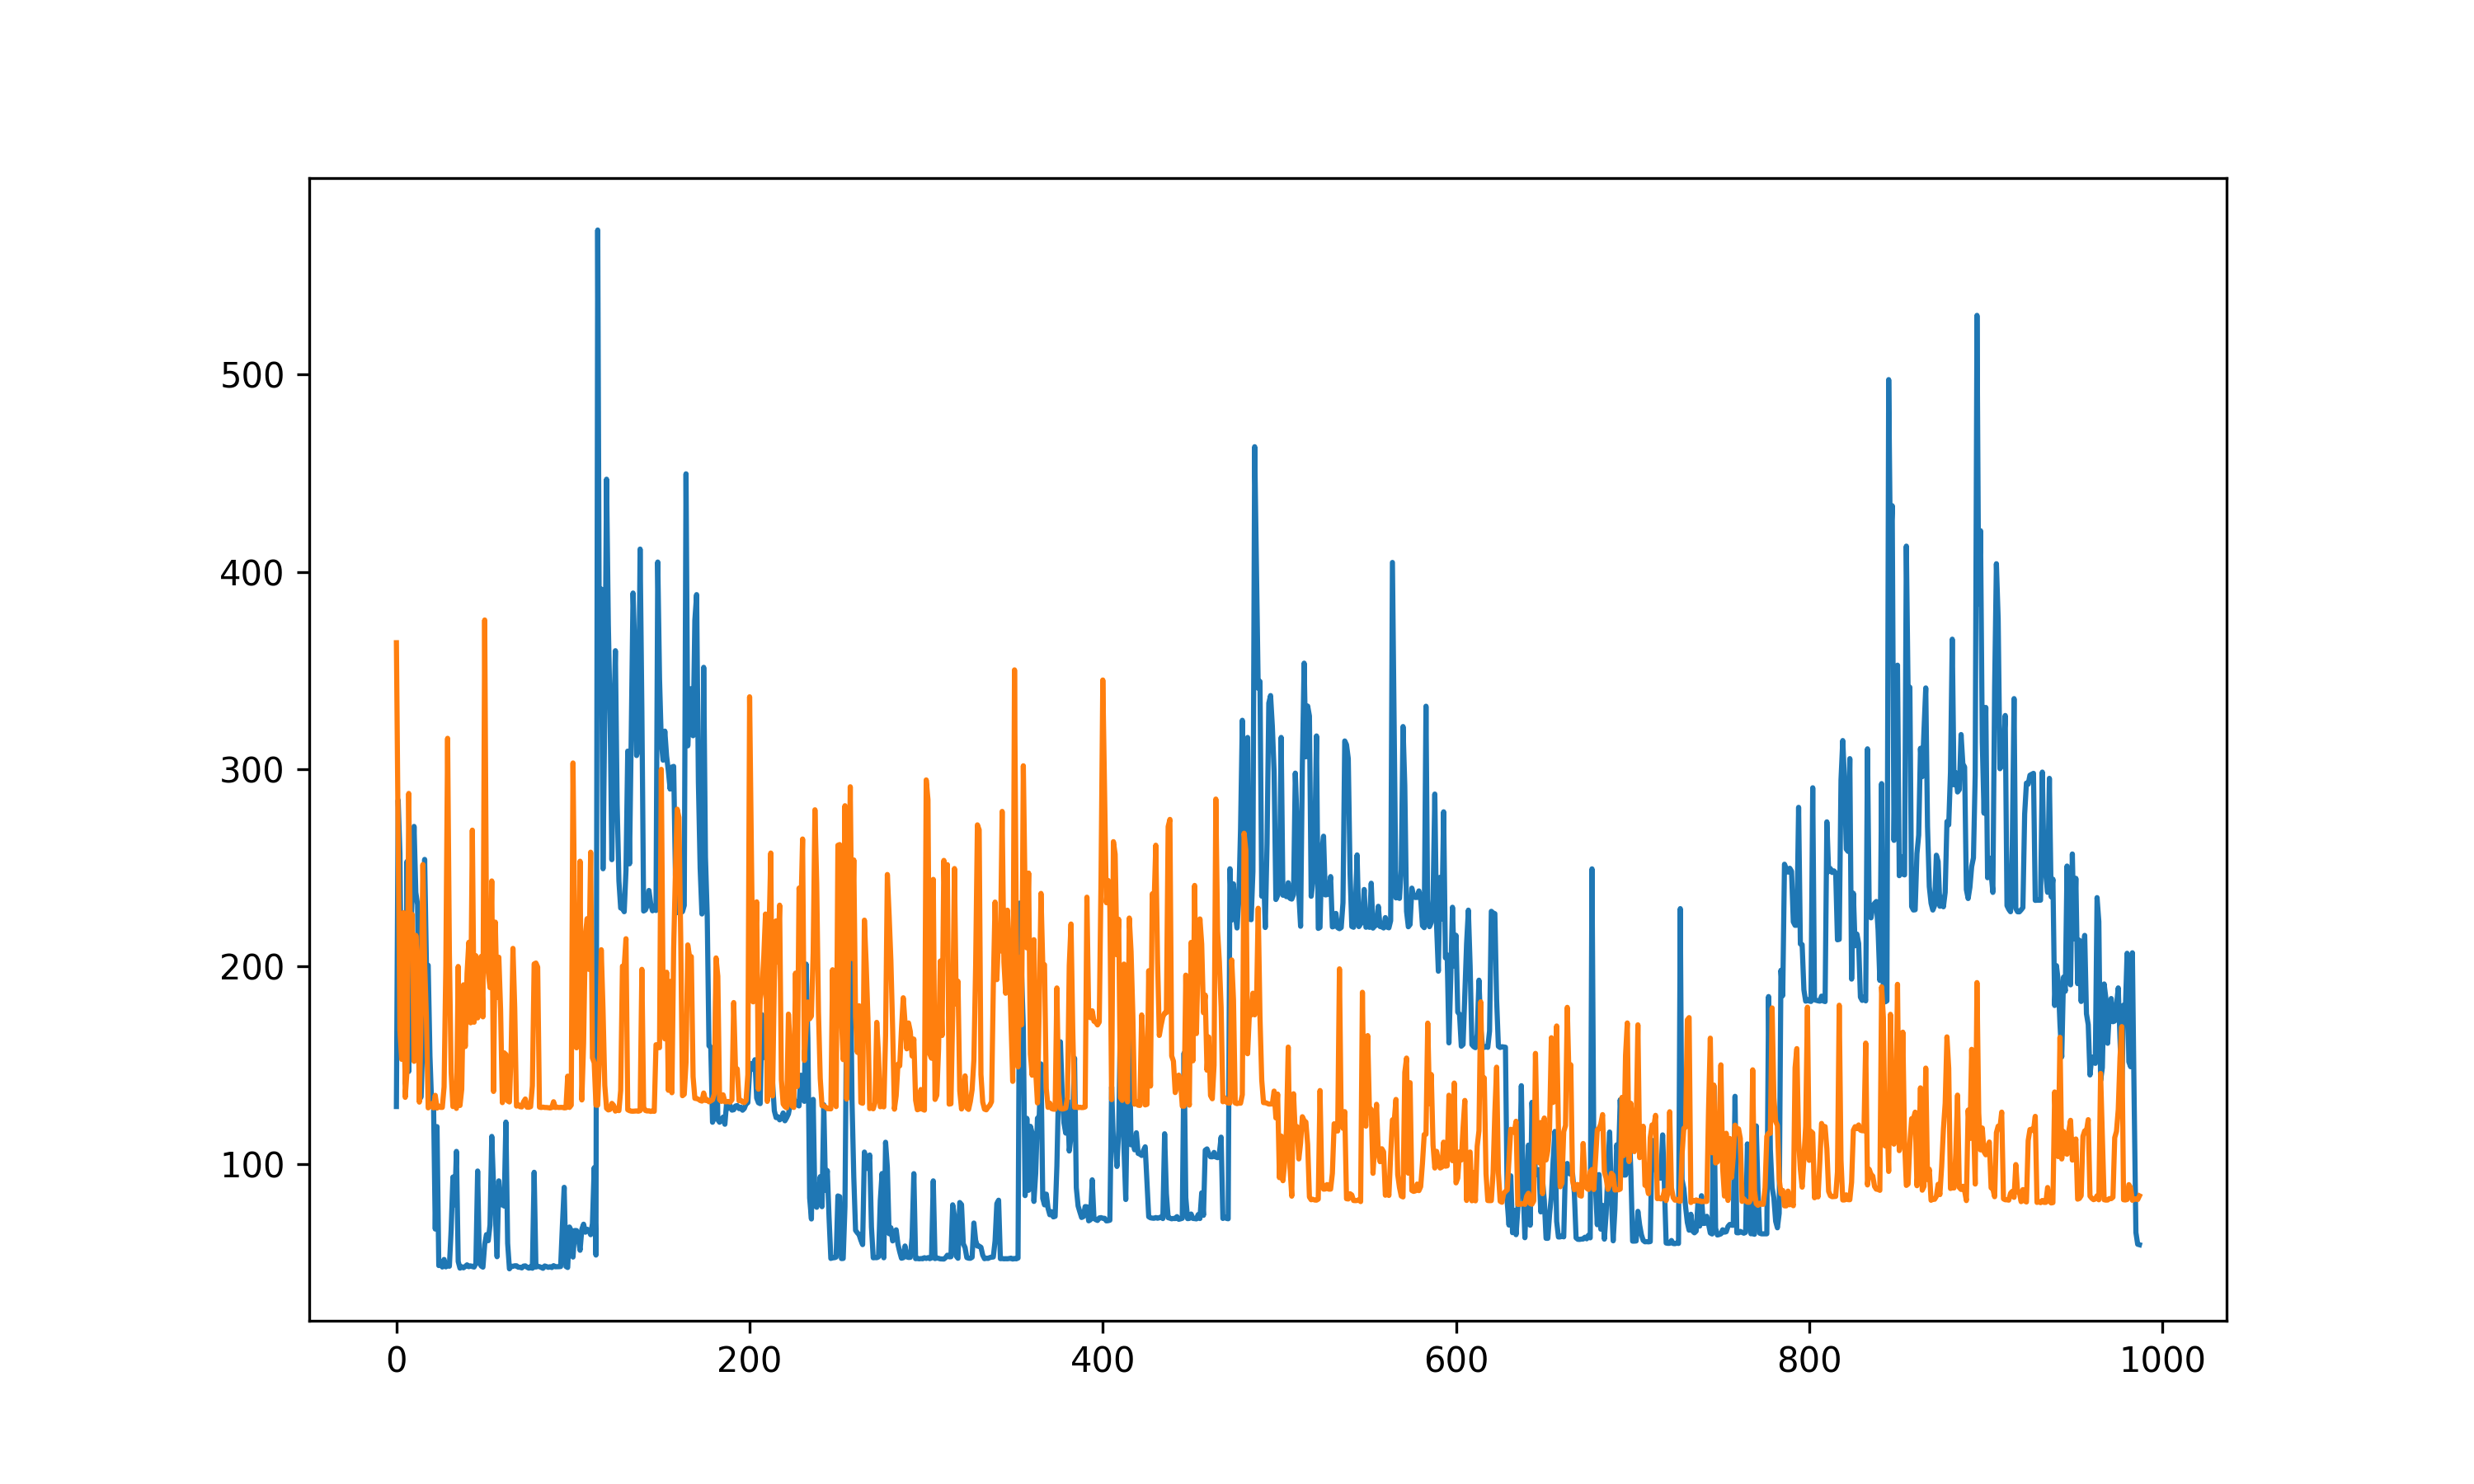
\includegraphics[width=1\textwidth]{plot_0.png}
    \caption{Benchmark 1 and 2 From sleeping Barber}
    \label{fig:mesh1}
\end{figure}


\begin{figure}[h!]
    \centering
    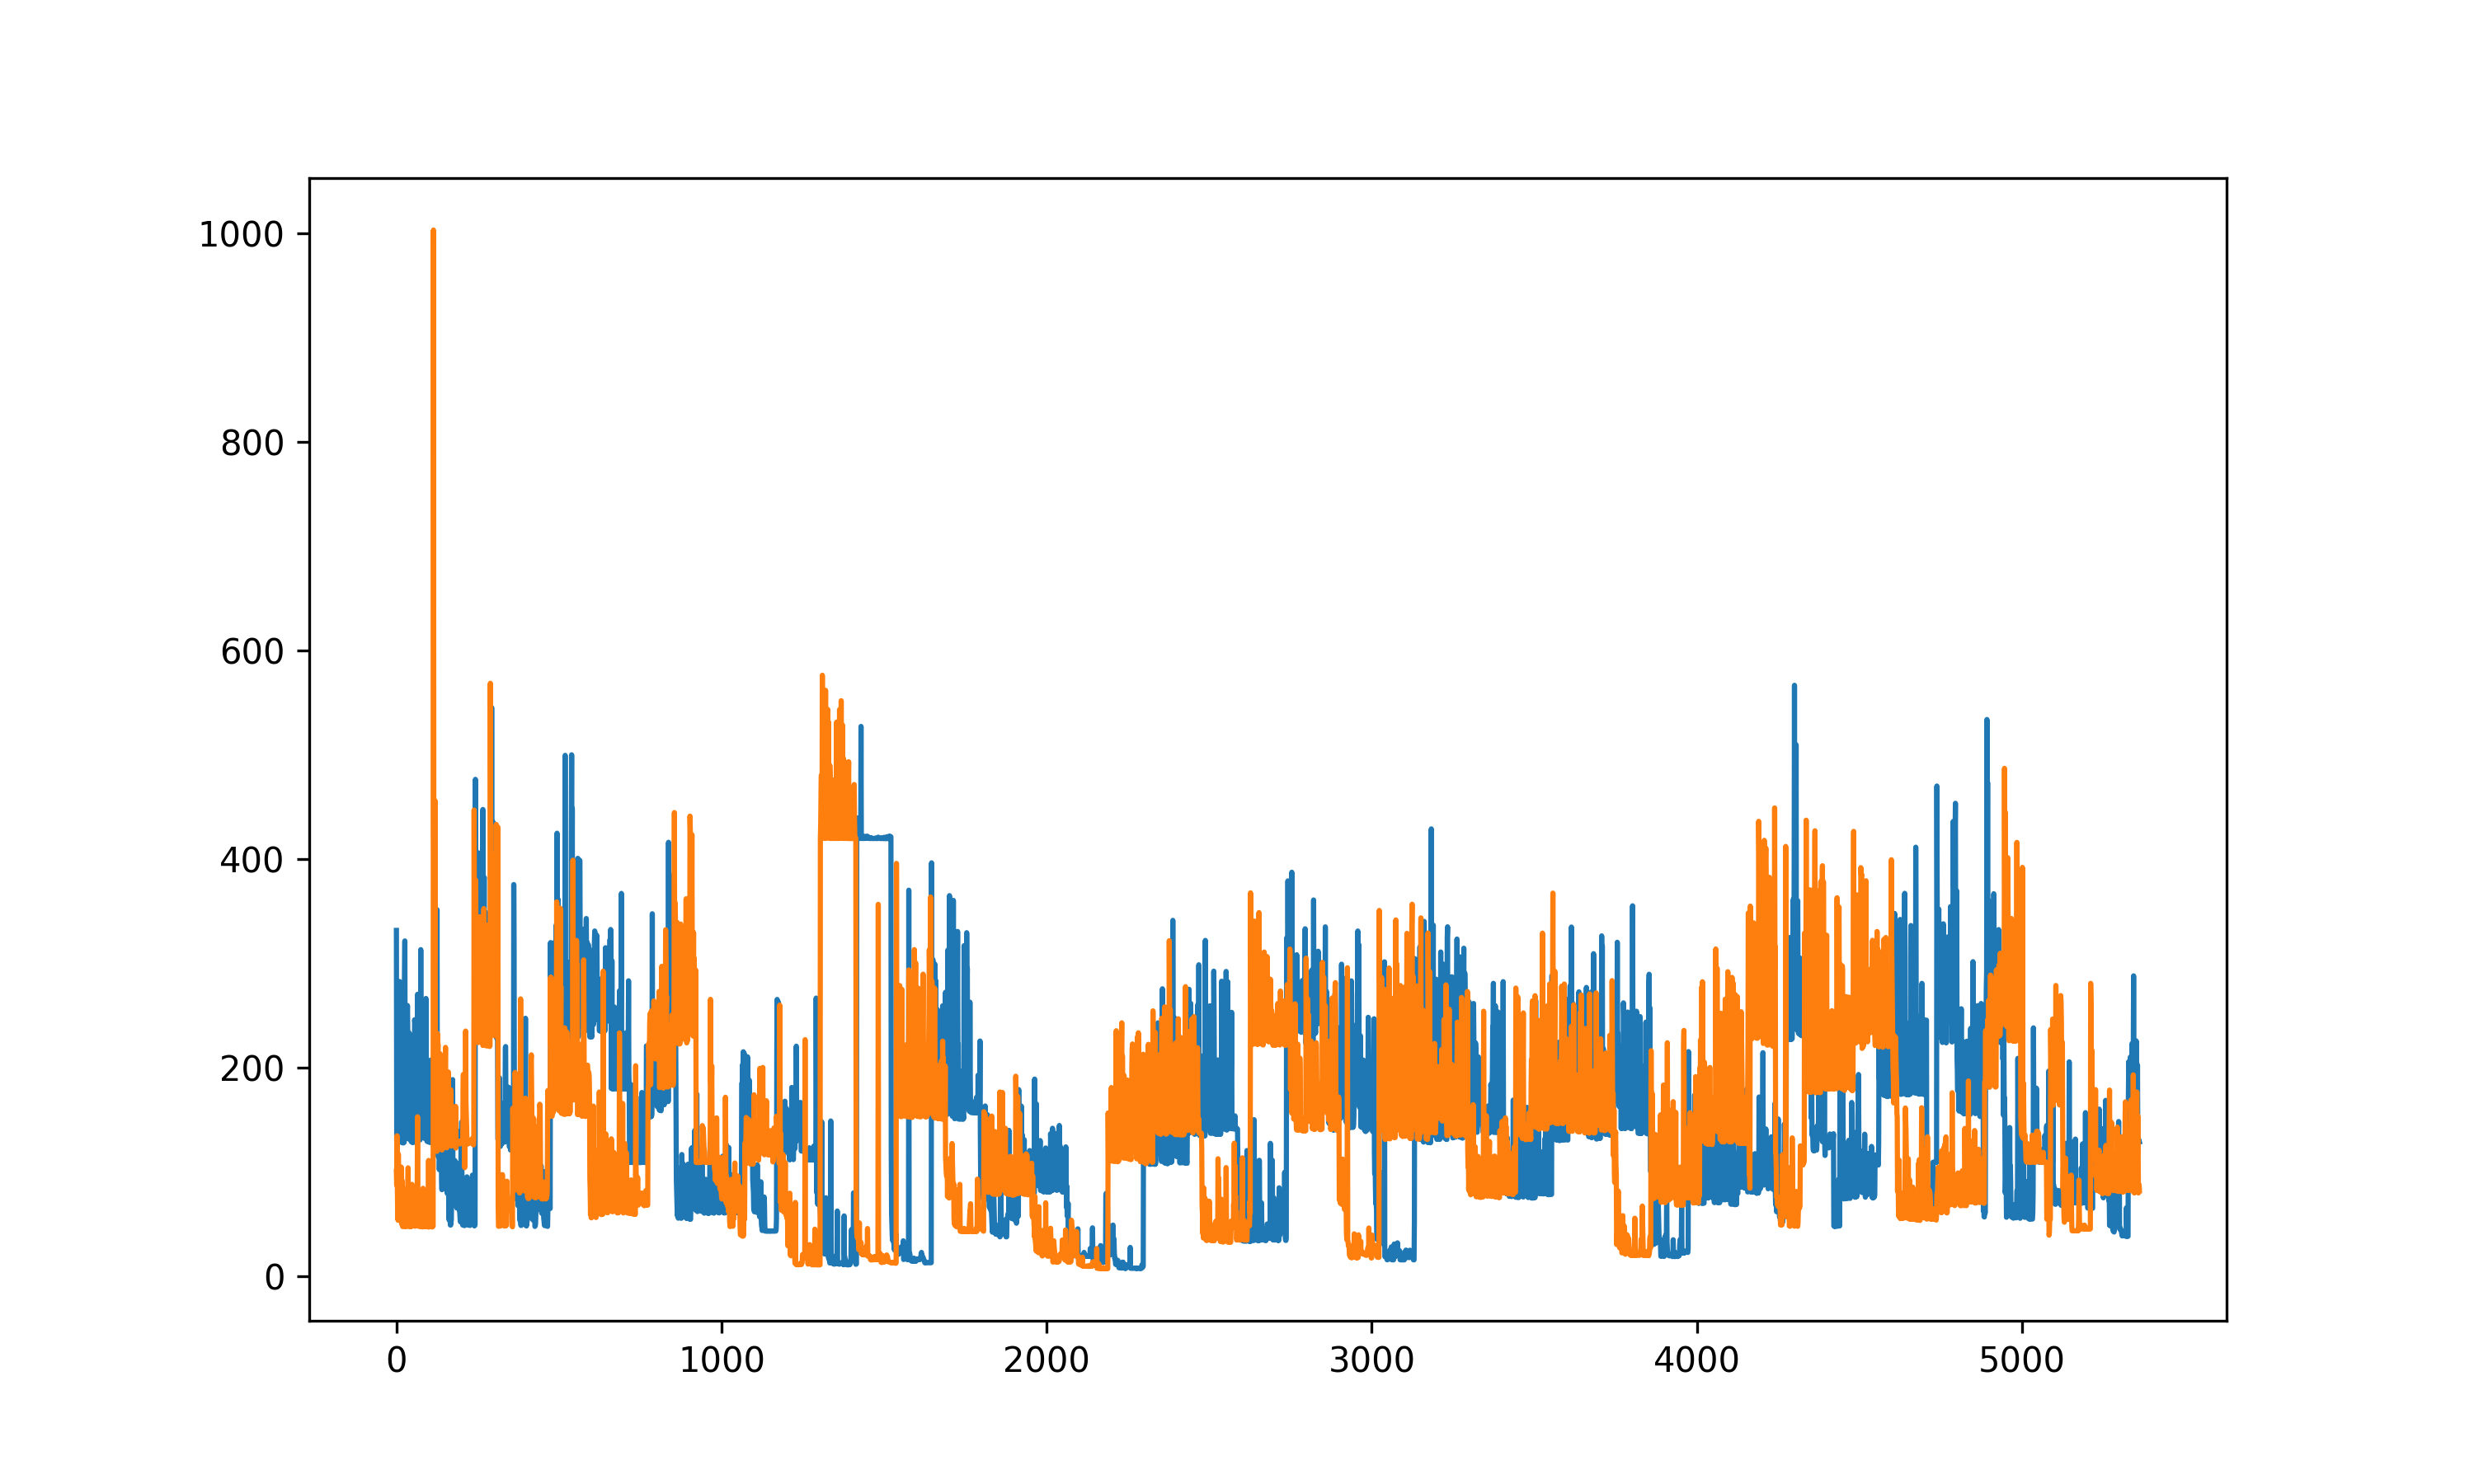
\includegraphics[width=1\textwidth]{plot_1.png}
    \caption{Benchmark 2 and 3 From sleeping Barber}
    \label{fig:mesh1}
\end{figure}

\begin{table}[h!]
\begin{tabular}{|l|c|c|c|c|c|c|}
   \hline
   benchmarks & pcm & frechet distance & area & curve length & DTW & directed hausdorf \\
   \hline
   1 \&  2 & 132 & 313 & 81918 & 14 & 68757 & 197\\
   \hline
   2 \& 3 & 573 & 295 & 32960 & 48 & 191649 & 7 \\
   \hline
\end{tabular} \\ 
\caption{Comparaison between two inequal benchmarks and two equal benmarks}
\end{table}


As expected the only algorithm that seems to work is the directed hausdorf algorithm because it is not influence by the size of the dataset, indeed as the curve lenght increase the difference of the score increase. 
I have put a treshold of 20 with the directed hausdorf. When the direcred hausdorf value is more than 20 is interesting to look at the benchmark because it means that their is significant difference between the two benchmarks.

\subsection{Conclusion of classification of changement of behaviour between benchmarks}

The validation of an unsupervised classification, as well as the choice of the number of group always remain open questions. On real data, recognized criteria such as the distance difference or the silhouette index are optimal with only two groups, limiting the contribution of such an analysis.





\bibliography{reference}


\end{document}
